\chapter{Experimental Observables in High-Energy Physics}
\label{ch:experiment}
\label{ch:chapter3}

Steering away from theoretical aspects, this chapter aims now at introducing key experimental observables from particle physics, which will be necessary for the study of vector leptoquark production under LHC conditions. The study presented throughout this dissertation involves simulations of proton-proton collisions at the LHC and the subsequent production of particles from the vacuum that interact with dedicated particle detectors. These simulations were performed using the geometry and experimental conditions of the Compact Muon Soleneoid detector, CMS. Therefore, some of the main features of this detector are described.

The detector has a cylindrical geometry as shown in figure \ref{fig:cms-detector}. It is $21.6\;\si{m}$ long and has a diameter of $14.6\;\si{m}$. Its total weight is $12500$ tonnes. The detector evinces a layered design, with different subdetectors and components in each layer. The innermost layer consists of pixel detector and silicon trackers. This layer enables the precise and efficient measurement of the trajectories of charged particles emerging from collisions. Surrounding this layer, are the electromagnetic (ECAL) and hadronic (HCAL) calorimeters. The ECAL uses lead tungstate (PbWO$_4$) crystals to efficiently absorb charged particles and transform their energy into a measurable signal. The HCAL has a similar operation. The next layer has a superconducting solenoid, which produces a large uniform magnetic field enabling the measurement of charged-particle momenta. Finally, the outermost layer is the muon detector system. It has the capability of reconstructing the momentum and charge of muons \cite{CMS_experiment}.

\begin{figure}[h]
    \centering
    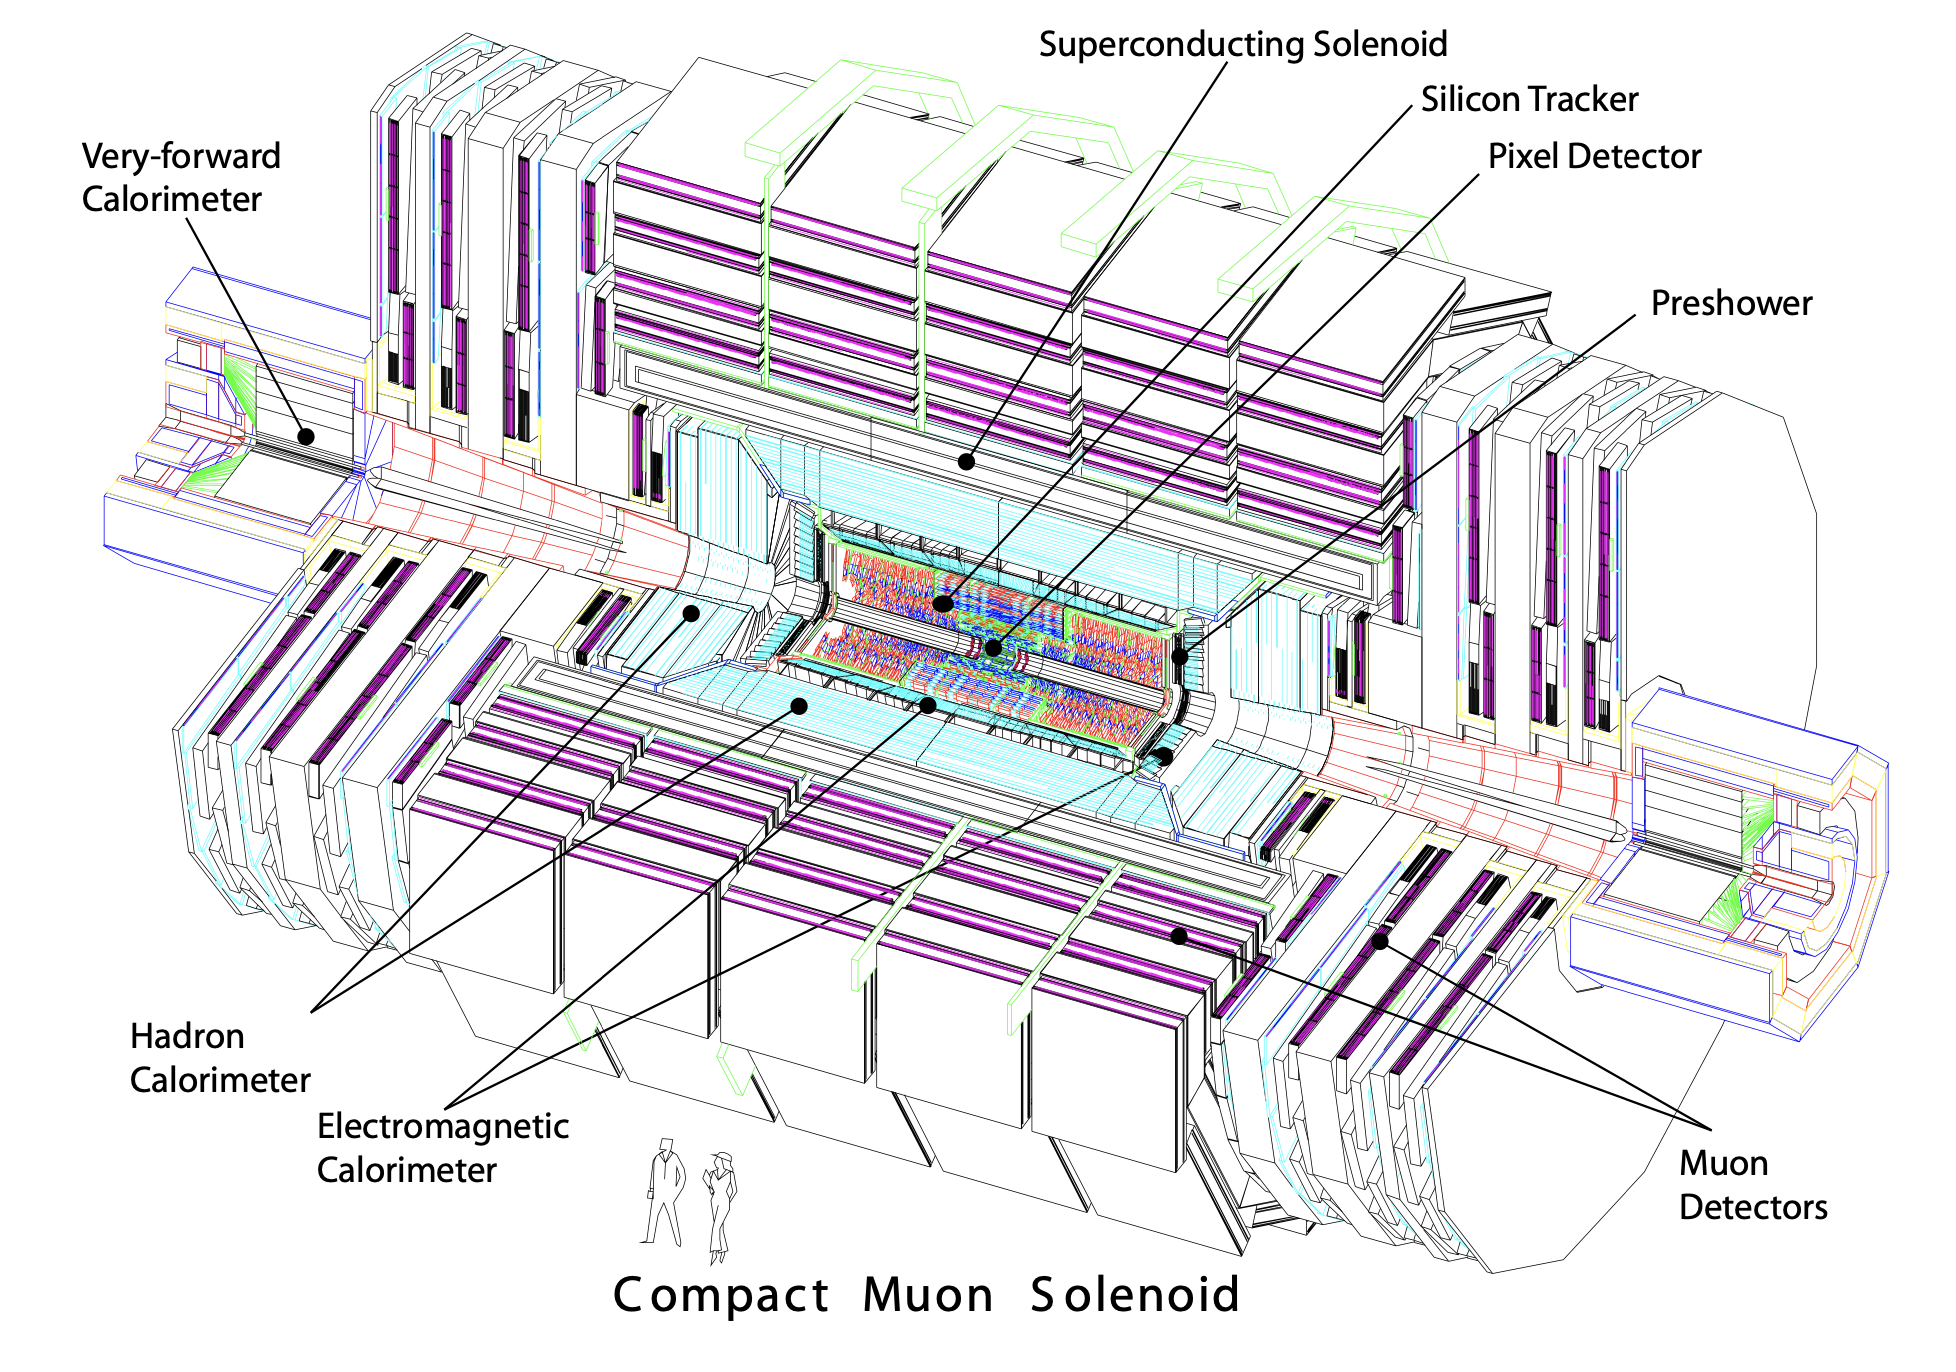
\includegraphics[width = 0.8\textwidth]{images/cms-detector.png}
    \caption{Diagram of the CMS detector showing inner components (retrieved from \cite{CMS_experiment}).}
    \label{fig:cms-detector}
\end{figure}

Measurements by the CMS adopt the coordinate system whose origin lies at the collision point, the $y$-axis pointing vertically upward, the $x$-axis pointing radially inward toward the centre of the LHC and the $z$-axis along the beam direction, towards the Jura mountains (see fig. \ref{fig:coordinate_sys}). The azimuthal angle $\phi$ is measured in the $xy$-plane from the $x$-axis and the polar angle, $\theta$, is measured from the $z$-axis.

\begin{figure}
    \centering
    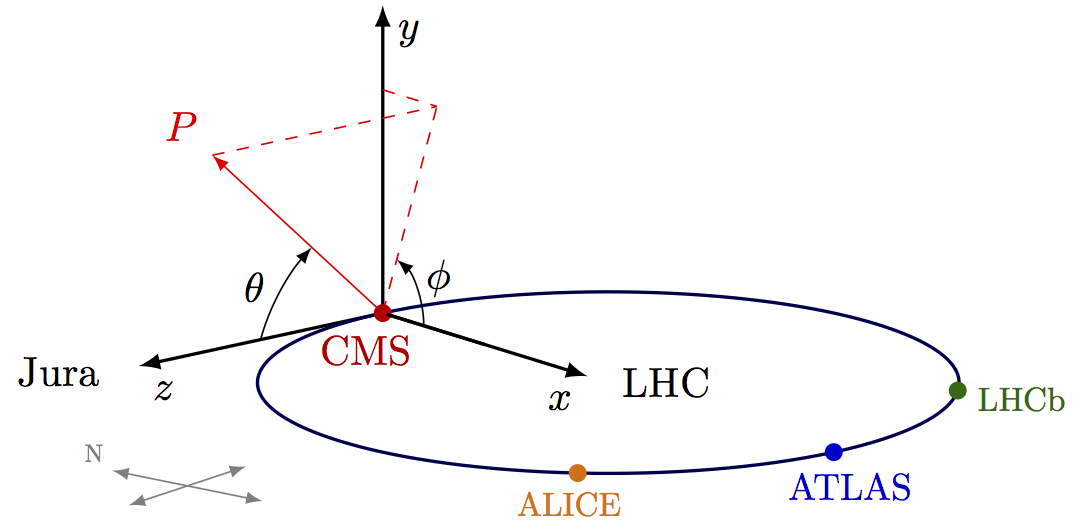
\includegraphics[width = 0.58\textwidth]{images/cms_coordinate_system.png}
    \caption{Coordinate system employed by the CMS experiment (retrieved from \cite{CMS-wiki}).}
    \label{fig:coordinate_sys}
\end{figure}

\subsubsection*{Experimental variables}
A key element of any experiment is the set of variables that will be measured. Thus, in order to fully describe the CMS experiment, some of its parameters should be outlined. The two most important parameters of an accelerator are the following:
\begin{description}
    \item[Luminosity ($\mathcal{L}$)] Measures the ability of an accelerator to generate interactions; it establishes a proportionality between the rate of interactions, $dR/dt$, and the production cross-section, $\sigma$ (defined below).
    \begin{equation}
        \dv{R}{t} = \mathcal{L} \sigma.
    \end{equation}
    For LHC beams, which collide head-on with a gaussian density distribution and come in bunches, the luminosity is given by $$\mathcal{L} = \frac{f N_1 N_2 N_b}{4\pi \sigma_x \sigma_y},$$ where $N_1$, $N_2$ are the numbers of particles in each colliding bunch, $f$ is the frequency at which bunches collide, $N_b$ is the number of bunches, and $\sigma_{x}$, $\sigma_{y}$ are the density deviations along the $x$ and $y$-axes, respectively \cite{herr-luminosity,thomson_modern_2013}.
    
    The luminosity can be integrated in time to obtain a direct relationship between event number and the cross-section:
    \begin{align}
        L = \int \mathcal{L}\, dt,\\
        N = L\sigma.
    \end{align}
    
    \item[Centre-of-mass energy ($\sqrt{s}$)] The energy of the colliding particles in the centre-of-mass (CM) frame. Since the total momentum of the particles in the CM frame is zero, the CM energy is simply the square-root of the total 4-momentum:
    \begin{align}
        \sqrt{s} = \sqrt{P^\mu P_\mu},\\
        P^\mu = \sum_{i} p^{\mu}_{i}.
    \end{align}
    The energy in the CM frame must be greater than the total mass of the particles being produced. Thus, the CM energy determines which particles can be studied in the accelerator.
    
\end{description}

The following variables are related to the particles being produced rather than the accelerator.
\begin{description}
    \item[Decay width ($\Gamma$)] The decay rate is the probability that a given particle will decay per unit time. Since a particle can suffer multiple decay modes, the total decay rate is the sum of the decay rates for each mode \cite{thomson_modern_2013}. The relative frequency of a decay mode is the \textit{branching ratio}, given by
    \begin{equation}
        \operatorname{BR}(j) = \frac{\Gamma(j)}{\Gamma}.
    \end{equation}
    
    \item[Cross-section ($\sigma$)] The cross-section is a measure of the probability that an interaction will occur from a collision. It is a quantum-mechanical analogue of the ``effective size'' of the particles involved in an interaction. It is related to the decay width according to
    \begin{equation}
        \Gamma = \rho\sigma v,
    \end{equation}
    where $\rho$ is the number density of particles and $v$ is the relative velocity of the incoming particles \cite{thomson_modern_2013}.
    
    \item[Pseudo-rapidity ($\eta$)] Instead of using the polar angle, CMS measurements involve the pseudo-rapidity, defined by
    \begin{equation}
        \eta = - \ln(\tan{\frac{\theta}{2}}).
    \end{equation}
    The main advantage of using the pseudo-rapidity is that distributions over it tend to be closer to a uniform distribution than those over the polar angle. Furthermore, the difference in pseudo-rapidity is invariant under Lorentz boosts along the beam direction \cite{thomson_modern_2013}.
    
    \item[Missing transverse energy and momentum ($E^{\mathrm{miss}}_T$ \& $p^{\mathrm{miss}}_T$)]
    Missing energy and momentum refers to the energy and momentum that is not detected but is expected to be there as a consequence of energy conservation and momentum conservation. This momentum is often carried by particles that do not interact electromagnetically or strongly and are therefore difficult to detect \cite{thomson_modern_2013}. Missing energy and momentum provides an indirect measurement of undetectable particles in hadron colliders such as neutrinos. Missing momentum reconstructions focus on the transverse direction, where total momentum is expected to be zero.
    
\end{description}